\documentclass[12pt,a4paper,oneside]{report}

\usepackage{amsmath}
\usepackage{mathtools}
\usepackage{mathrsfs}
\usepackage{parskip}
\usepackage{graphicx}
\usepackage{hyperref}
\DeclareGraphicsExtensions{.png}

\begin{document}
\title{Honours Dissertation: Semi-Supervised Learning on Data Streams}
\author{Michael Glenny}
\date{October 28, 2014}
\maketitle

\section{Introduction}
\section{Related Work}
\section{Label Stream: An Algorithm for Classifying Stream Data}

The algorithm that I chose to attempt to improve was one developed by researchers at the University of Dallas. The Label Stream algorithm was published in 2009 by Clay Woolam, Mohammad M. Masud and Latifur Khan.\cite{LabStr}

The basic framework of the algorithm is to use an ensemble of models to predict which class a data point belongs to. The stream is broken into chunks, and each model is built from the data in a partially labelled chunk. When a new model is created, we simply need to update our ensemble by evicting the model which is performing worst on the new labelled data, as well as refining the current models in the ensemble based on the labelled data seen in the new chunk. 

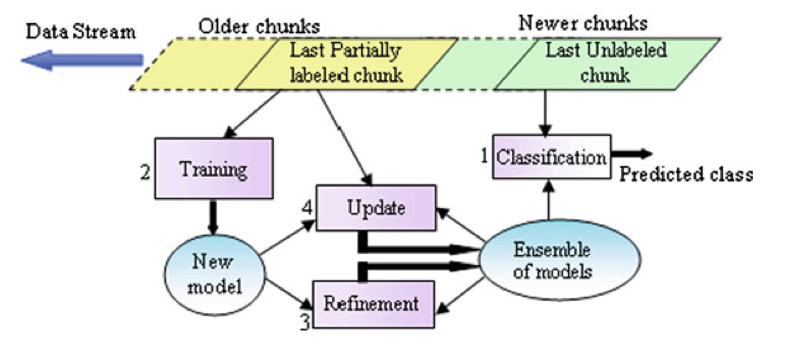
\includegraphics[scale = 0.4]{LabStrOverview}
\cite{TechRep}


\section{Training a Model}

We can train a model from a data chunk as soon as some arbitrary percentage of the data points in that chunk have been manually labelled. Experimental testing by Woolam et al. shows that Label Stream performs as well as many previous stream classification algorithms with as few as \(10\%\) labelled points.\cite{LabStr}

Training a model based on a chunk of data consists of three steps. Firstly, we cluster the data into large macro-clusters based on a modified version of K-Means clustering, in which we try not only to minimise intra-cluster distance like in standard K-means, but also minimise cluster impurity by taking into account the entropy of clusters as a dissimilarity measure in which clusters with points of different labels are punished. 

Secondly, we then split those macro-clusters into class label pure micro-clusters. Some of these micro-clusters will be unlabelled, and hence the third step is to use a Label Propagation technique to label the unlabelled micro-clusters. Now that all the micro-clusters are labelled, they are ready to be used in the classification process. 

\subsection{The Macro-Clustering Step}

\subsubsection{MCI K-Means}
 In regular K-means clusters, we wish to minimise the intra-cluster distance in every cluster, which can be expressed  as minimising an objective function: 
 
 \[ O_{Dist} = \sum_{i=1}^K \sum_{x\in X_i}|| x - \mu_i||^2 \]
 
This is an unsupervised technique, but we would like to take advantage of the fact that a certain percentage of our data chunk have labels associated. To do this, we will modify unsupervised K-means by adding an additional factor to the objective function. This is called by Woolam et al. MCIK-means, which stands for Minimising Cluster Impurity for K-means. \cite{LabStr} The objective function for this variation on K-means is:
 
 \[ O_{MCIKMeans} = \sum_{i=1}^K \sum_{x\in X_i}|| x - \mu_i||^2(1 + Ent_iADC_i)\]
  
Firstly, we need to define entropy. Entropy is a measure which is normally used to describe how many bits are necessary to convey information, but is useful in this context as a measure of purity of clusters. The formula for calculating the entropy of a cluster \(i\) is:
 
\[Ent_i = \sum_{c=0}^C(-p_i^clog(p_i^c))\] 

where \(p_i^c\) is the prior probability of a point in the cluster \(i\) being of class \(c\), i.e.:
\[p_i^c = \frac{|X_i(c)|}{|X_i|}\] 

Entropy will give a higher penalty to impure clusters, however using only entropy will mean that every point has the same penalty related to impurity. This is a problem when we try and minimise our cluster impurity. Suppose for instance we have cluster A, with 9 points of label 1, and cluster B, with 3 points of label 1. Then, suppose we add 7 points of label 2. 

The best arrangement we can hope for is for cluster A to remained untouched, and cluster B to take all the points of label 2, resulting in an entropy of 0.26. However, what will happen when we incrementally add each point? Well, in the first instance, because cluster A is larger, a point of label 2 will be assigned to it. Now because cluster A is impure, we will continue adding points to cluster A, and our final configuration will be cluster A with 16 points in total, 9 of class 1 and  7 of cluster 2, and an entropy of 0.29, and cluster B as it was with an entropy of 0. This is not the optimal configuration!

To solve this problem, we introduce a measure of cluster impurity called Dissimilarity Count. We define the dissimilarity count of a point \(x\) in a cluster \(i\) to be:

\[DC(x,i) = \sum_{c=0}^C(|X_i| - |X_ic|)\] 

Basically, the dissimilarity count of a single point is the number of points in the cluster with a class label other than the class of that point. In our previous example, using Dissimilarity Count, we would place all the points of label 2 into cluster B, because the dissimilarity count for all points of label 2 would stay the constant 3, for all the points of label 1 which were there before. 

The Aggregated Dissimilarity Count, ADC, is simply the sum of all dissimilarity counts for each point in a cluster. 

/* A graph demonstrating the above examples would help */

An outstanding issue is whether to consider unlabelled points as a distinct class or not. In the original Label Stream paper, it is clear that unlabelled points are not to be considered in the Dissimilarity count, as they explicitly state that if a point is unlabelled, \(DC(x,i) = 0\).\cite{LabStr} However, in Khan et al. review of the same algorithm, it is more equivocal, and the paper seems to suggest that they did consider unlabelled points as a distinct class for the purposes of calculating the dissimilarity count. For my experiments, I have decided to uphold the convention of the dissimilarity count of an unlabelled point being zero.  
 
 \subsubsection{Expectation Minimisation} 
 In order to generate these clusters, firstly we need to initialise our clusters. This initialisation can be have a great effect on the quality of the subsequent clustering. Firstly, we take all the labelled points in our data chunk and calculate the prior probability of a certain class appearing in that chunk. Then, for each class, we calculate the proportion of the K clusters to be generated which should be initialised to a point of that class. This calculation is:
 
Number of clusters initialised to class \(i  = p_i^cK\) 

where K is the number of macro-clusters. Now, we use the furthest apart initialisation method to select the points which will be the centroids of our macro-clusters. That is, we find the point of class \(i\) which is furthest away from all the points in \(i\) which have already been selected as centroids for clusters. Masud et al. report that this method of initialisation, proportionate to the distribution of labelled data in the data chunk greatly improved their cluster quality.\cite{TechRep}

With the clusters initialised, we can now apply Expectation Minimisation to find a clustering. Firstly, we apply the E-step, in which we assign a point to the cluster which minimises the contribution to the global function, regardless of whether that point is already assigned to a cluster or not: 

 \[O_{MCIKMeans}(x) = || x - \mu_i||^2(1 + Ent_iDC_i(x)) \]
 
The value of the overall objective function depends on the order by which we add points from the chunk to the clusters. If we were to attempt to try all possible orderings of points, this step would be computationally intractable. Instead, we can randomly shuffle the points. This will not guarantee that the cluster converges to the global minimum for the objective function for MCI K-means, but the algorithm will converge in relatively few iterations. 

The Minimisation step is to simply recalculate the centroid of each cluster, \(\mu_i\), by averaging all the points now in that cluster. The calculation for that step is: 

\[\mu_i = \frac{\sum_{x \in X_i}x}{|X_i|}\]

We then repeat these steps until the convergence condition is met. We consider the algorithm to have converged if no single point has changed cluster after the point re-assignment phase. This idea of shuffling points randomly and this convergence condition is called the Iterative Control Method, which is guaranteed to converge.\cite{ICM}  
 
 \subsection{The Micro-Clustering Step}
 
Once the macro-clustering step is complete, we will have \(K\) macro-clusters which may or may not be class pure. Our next step is to break these macro-clusters into micro-clusters which are class pure. The procedure is rather simple based on what is considered 'pure':

\begin{enumerate}
\item Firstly, if a macro-cluster only contains labelled points from a single class, then it is already pure, and we can consider that macro-cluster as a micro-cluster. 
\item Secondly, if a macro-cluster contains labelled points from two different classes, then we split that macro-cluster into two micro-clusters where each micro-cluster will only contain points from one class. 
\item Thirdly, if a macro-cluster contains labelled points from one class as well as unlabelled points, we will split these points into two micro-clusters, one with the labelled points, and with unlabelled points. 
\item Fourthly, if we have a micro-cluster which only contains unlabelled points, we will further subdivide that micro-cluster into micro-clusters based on the predicted class labels of those unlabelled points.  
\end{enumerate}

The reason we split these macro-clusters into micro-clusters is so that we can make definitive statements about the labels of the labelled micro-clusters. If this is the goal of the splitting, we might ask why we split unlabelled micro-clusters based on their predicted classes. If an unlabelled micro-cluster is constituted of two underlying classes, which have some geometric division, hopefully our predictions from previous models will be able to detect this. If we can successfully split this micro-cluster, the quality of our label propagation will increase greatly. An example is given in this figure taken from Woolam et al.\cite{LabStr}

\includegraphics[scale = 0.7]{ClusterSplitting}

Once we have finally decomposed our macro-clusters into micro-clusters, we won't store the complete micro-cluster, because we have no use for the complete listing of points in the micro-cluster. In the Label Stream algorithm, three basic pieces of information are stored about the micro-cluster. However, at this point, we will calculate a measure of cluster quality based on the LoOP measure, explained later:
\begin{enumerate}
\item The centroid of the micro-cluster, \(\mu\)
\item The weight of the micro-cluster, which is simply the number of points it contains, \(\rho\)
\item The label of the micro-cluster. If the micro-cluster contains only unlabelled points,  
\item In addition, we will store the LoOP score of the cluster. 
\end{enumerate}

This summary of the micro-cluster is called a pseudo-point. However, at the moment, all the micro-clusters which had no labelled points in them have no label! Hence, we move on to the third phase of our label propagation. 

\subsection{Label Propagation}

In order to label our unlabelled micro-clusters, we will use a label propagation technique originally devised by Zhou et al.\cite{LabProp}. Their basic technique is to build a complete graph where each micro-cluster is and each edge is a measure of weight or influence that one micro-cluster has on another. The influence in that technique that \(i\) exhibits on \(j\) is based on the Gaussian Kernel Function:

\[W_{i,j} = e^{-(\frac{||x_i-x_j||}{2\sigma^2})}\]

Where \(x_i\) and \(x_j\) are the centroids of micro-clusters \(i\) and \(j\), respectively, and $\sigma$ is standard deviation. 

To modify this affinity matrix, as it is called by Zhou, to suit our purposes, we simply need to change this undirected complete graph into a directed complete graph where \(W_{i,j}\) represents the weight or influence that \(j\) exerts on \(i\). The reason the influences will not be symmetric is that the influence \(j\) exhibits on \(i\) will now be proportional to the weight of the micro-cluster, i.e. the number of points in the cluster. This equation can be expressed as:
\[
	W_{i,j} =
	\begin{cases}
	 e^{-(\frac{||x_i-x_j||}{2\sigma^2})}\rho_j : i \neq j \\
	0 :					 i  = j 
\end{cases}\] 

We use this function to generate the affinity matrix. Note that if $i$ and $j$ are equal, we set the affinity matrix to be zero. When we construct our affinity matrix, we include in addition to the micro-clusters generated in this mode, labelled micro-clusters from a number of the most recent models built, so that we have a large amount of labelled data to use in our label propagation. For our experiments, we have set the number of previous models to contribute labelled micro-clusters to be 3.

We now need to normalise this affinity matrix. We will do this by taking the Normalised Laplacian of the affinity matrix. The equation for this normalisation is:

\[ \mathscr{L} = D^{-1/2}LD^{-1/2}\] 

Where $L$ is the affinity matrix we built before,  $D$ is a matrix analogous to the degree matrix in a discrete setting.$D$ is a diagonal matrix where the diagonal entries are the sum of the rows of the affinity matrix, and zero otherwise. This can be expressed as:
\[
	D_{i,j} =
	\begin{cases} 
	 \sum_{x} L_{ix} : i = j \\
	0 :					 i  \neq j 
\end{cases}\] 

Since this matrix is diagonal, taking the inverse and square rooting the matrix is as simple as taking the inverse of each diagonal element and then taking the square root.

Before we apply the label propagation, we need to construct a representation of the labels of our micro-clusters. We will call this matrix $\Upsilon$ We will generate a $C$ by $M$ matrix, where M is the number of micro-clusters. For micro-cluster $m$, if it is unlabelled, the $m$th row will contain only zeros. If $m$ is labelled, and of class $c$, then this matrix will a 1 at $\Upsilon_{mc}$.

Let this initial state of $\Upsilon$ be $\Upsilon^{(0)}$. Now we can let the labels of the $\Upsilon$ matrix propagate though our complete directed graph using the affinity matrix. The equation with which this happens is:

\[ \Upsilon^{(n+1)} = \alpha \mathscr{L} \Upsilon^{(n)} + (1 - \alpha) \Upsilon^{(0)}\] 

Here, $\alpha $ is the learning rate, which we set of 0.99 in our experiments as suggested by Masud et al.\cite{TechRep} The label of a given micro-cluster $m$ at convergence is the column at which the value of $\Upsilon_{mc}$ is greatest. The convergence condition on the label propagation is the point where no micro-cluster changes its label over subsequent iterations. 

\subsection{Using a Model to Classify a Point}

In order to classify a given point against a single model, we build a vector $Y$with $C$ elements, where $Y_c$ represents a score for that point being of class $c$. To generate this score, we simply use the Gaussian Kernel Function to score the distance between the point and every micro-cluster, and then add that score to $Y_c$ where $c$ is the label of that given micro-cluster. We will also, after comparing the point to every micro-cluster, normalise the vector, with a small non-zero epsilon to avoid dividing by zero. This process can be expressed as an equation for labelling point $x$:

\[ Y = \frac{\sum_j(W(x,\mu_j))Lab_j}{\sum_j{W(x,\mu_j)} + \epsilon} \]
where
\[W(i,j) = e^{-(\frac{||x_i-x_j||}{2\sigma^2})}\rho_j\]

To classify the point against this model, we simply label the point as class $c$ where $c$ is the index with the largest value in $Y$.
\section{Classification and the Ensemble}
 
An ensemble is a collection of Models which we use to classify points in our stream. We use an ensemble to classify points in the data stream rather than the most recent model for several reasons. Firstly, because a single model is trained on only a small subset of the dataset, a certain model can be poorly trained. In this case, our poorly trained model will be quickly evicted from our ensemble. 

Secondly, the ensemble is an excellent way to handle concept drift within a stream. If there is a concept shift within the stream, models trained after the concept shift will gradually replace those models trained beforehand, and slowly the classification decisions of the ensemble will adapt to the concept drift. If however, a certain change in distribution of data in a chunk is cause by random chance and is not a genuine concept drift, the model trained with that data will simply be evicted as soon as the data distribution returns to normal. 

\subsection{Adding a Model to the Ensemble}

Once we have generated a model, we will need to include it in our ensemble of Models, which we will use to classify points. There are, however, certain steps we need to execute whenever we add an model to an ensemble. Firstly, we need to add our new model to the current ensemble. If our ensemble is not full, then we simply add it without any modification. However, if our ensemble is full, we need to evict our worst performing model. We do this by taking the labelled points in the data chunk used to train the most recent model (i.e, the most recent labelled points) and scoring the performance of each model in the ensemble. If two models perform equally well, we remove the oldest model.

\subsection{Handling a new Class in the Data Stream}

As we process the data stream, we may have a new class appear in the data stream that has never been seen before. This could be because our manual classifier felt that an examined data point could not be described within the current class framework. Woolam et al\cite{LabStr} call this an 'evolved class'. On the other hand, this could be a very rare class which has always existed in the data stream, but by chance has only now appeared. This raises the issue of what should be done about this new class. 

Since previous models do not know about this new class, it is not possible that previous models can predict it. So what we will do is inject a micro-cluster representing that point into the previous models, giving them a chance to predict the point when they are being evaluated for quality when a new ensemble is added. So, for any class which has never been seen before in the stream, we will add a micro-cluster to each model in the ensemble of that class. 

However, doing this repeatedly would inflate the number of micro-clusters in each model, and possibly inflate the complexity many of our processes. So to compensate, for every injected micro-cluster, we will find the two micro-clusters in each model which are of the same label and closest together, and merge them. This merging consists of removing both micro-clusters and creating a new micro-cluster where the centroid is the average of the old centroids, and the number of points is the sum of the number of points in both clusters. If we have so many classes that each micro-cluster in a model has a distinct label (and hence, no point can be merged), then we have violated the rule of thumb that the number of macro-clusters K should be greater than the number of classes in the data stream. 

Hence, we merge the nearest two micro-clusters only if:

\begin{enumerate}
\item There exists two micro-cluster of the same label
\item The total number of micro-clusters, \( M_i \geq K \), the number of macro-clusters. 
\end{enumerate}

There is the issue of whether injecting models with the new class and merging the closest pair of micro-clusters of the same label increases the classification accuracy. One the one hand, we might think the accuracy increases because no model without information on the class can predict a point of that class. However, injecting a micro-cluster into all of the models of the ensemble could increase the correlation between each model, reducing the overall accuracy of the ensemble. \cite{Inject}

The theory behind this injection is given a full discussion in Khan et al. \cite{TechRep}, and I will not repeat it here. The key finding is that as long as single model error decreases monotonically as the prior probability of the evolved class increases, our injection will always improve the quality of the ensemble classification given that our ensemble is not too large. This conclusion is drawn by proof incorporating a proof included in Turner et al.\cite{Inject}

\subsection{Removing Harmful Micro-Clusters from Models}

When updating our ensemble, we also attempt to remove micro-clusters from models which may have a negative impact upon the classification accuracy of our ensemble. 

This may seem like a tricky task, however a very clear theory for dealing with this problem is presented by Woolam et al.\cite{LabStr}. Firstly, we introduce the notion of a swing voter. A swing voter is a micro-cluster which determines which class a point to be predicted $x$ will be classified as: such that if that micro-cluster were a different label, then that point would be classified differently. It is asserted that such a micro-cluster must exist, and usually, it will be the micro-cluster which has the greatest value on the inductive label propagation function, $W(i,j)$.

Lets say that the probability a micro-cluster $m_i$ is a swing voter for a test point is $\alpha_i$. So for instance if $\alpha_i = 0.5$ that means that if there are 100 test points, then $m_i$ is the swing voter for 50 of them. Also, suppose we know the real class of a certain test point. Let $p_i$ be the probability that for micro-cluster $m_i$ and the test points for which it is the swing voter, the test point has the same label as $m_i$. So if $p_i$ is 0.5, then for the 50 test points for which $m_i$ is a swing voter, only 25 of them have the same label. 

Using this framework, we can say that a point $x$ is not misclassified because of a certain micro-cluster $m_i$ if:
\begin{enumerate}
\item $m_i$ is not a swing voter, or
\item $m_i$ is a swing voter and the class of $x$ and $m_i$ are the same.
\end{enumerate}

The probability of the first case is $(1-\alpha_i)$ and the probability of the second is $(\alpha_i(1-p_i))$. Hence, the probability of a certain micro-cluster ensuring a point is mislabelled is $1-\alpha_ip_i$. This means the probability that the next $N$ test cases are not mislabelled due to $m_i$ is $(1-\alpha_ip_i)^N$, and the chances of a single point being mislabelled due to $m_i$ is $1-(1-\alpha_ip_i)^N$. The expected classification error for a whole model is: $(1-\sum a_i(1-\alpha_ip_i)^N)$.

This means that if we want to reduce the classification error for the whole model, we can either reduce $\alpha_i$ or reduce $p_i$. In fact, it is this reasoning that led us to split unlabelled micro-clusters in the clustering step: by splitting the micro-cluster, we essentially replace one cluster with high $p_i$ with two with low $p_i$. 

However, if we were to attempt to reduce $\alpha_i$, we could do that by removing all micro-clusters! But that would preposterous. Instead, what we will do is keep track of micro-clusters which have high $p_i$, and if they become too high, we will simply remove them. This should improve the model classification accuracy, because for that micro-cluster, $\alpha_i = 0$ and so it will not cause any misclassification. However, this improvement only occurs if there is no cascading effect. If we remove a certain micro-cluster, now adjacent micro-clusters are swing voters for the points for which our deleted micro-clusters were swing voters. This may or may not lead those micro-clusters to be eligible for deletion. If we continue at this rate, then most or all of the micro-clusters could be deleted. 

Unfortunately, there is no tidy theory to deal with this problem. For our purposes, there is a hard limit of micro-clusters eligible to be deleted. Woolam suggested a threshold of no more than 50$\%$ point deletion, however here we allowed arbitrary deletion until the number of micro-clusters is no more than $K$, the number of macro-clusters in a model. 

\section{Using LoOP to evaluate cluster quality}

The previous sections lay out the Label Stream algorithm in its entirety. However, if we are to somehow attempt to use cluster quality measures to increase the classification accuracy of the algorithm, we need a method of evaluating the quality of the micro-clusters we generate. If we could score each micro-cluster based on its quality, then we could weight its contribution to the classification of the point, and hopefully achieve a better classification accuracy. 

Cluster evaluation methods typically use two basic measures. These are intra-cluster density, and inter-cluster separation. For example, Moulavi et al\cite{DBCV}. recently released a paper in which they evaluate cluster quality by scoring a cluster based on these two measures. To evaluate intra-cluster density, they score a cluster as the longest edge in a minimum spanning tree of the cluster, and evaluate the inter-cluster distance by finding the nearest pair of points between two clusters. They can then build an overall score based on these two measures. 

However, evaluating the quality of micro-clusters should not use inter-cluster measures. This is because cluster overlapping is not necessarily a sign of bad clustering. If we take a macro-cluster which contained labelled points of a class, and unlabelled points which are actually of that class, then we will split that cluster into two different micro-clusters at the micro-clustering phase. However, these overlapping clusters are not a problem because they both come from the same underlying class distribution. 

Another viable method to change the micro-clusters is simply to find outliers in a cluster and remove them. Since our clusters centroids are mean based, an outlier in a small cluster can skew the centroid of a cluster significantly. Identification and removal of these points maybe another way 

In this section, we will discuss LoOP, a method which evaluates how likely it is a single point is an outlier within a cluster. After we have explained how this measure works, we will look at how it can be applied to this problem. 

\subsection{LoOP: The Local Outlier Probability Factor}

When trying to determine whether a point is an outlier, many outlier scores only give an arbitrary score which must be interpreted. However, LoOP is innovative in the way that rather than producing an arbitrary score, each point is assigned a probability of being an outlier. This makes the results much easier to interpret. 

The first step is to define a probabilistic distance. Suppose we have a distance measure like euclidean distance, which we denote as $d(x,y)$. Suppose also we have some point we are interested in $o$, and a set of objects $S$. Then we want our probabilistic distance between two a point $o$ and the set of objects $S$ to be have the property:

\[\forall s \in S: P[d(o,s) \leq pdist(o,S)] \geq \phi\]  

where $\phi$ is some constant. Intuitively, what this means is that a sphere around $o$ with a radius $pdist(o,S)$ covers any element in S with probability $\phi$. Now, if we wish to estimate probabilistic density, we can take the inverse of the $pdist$:
\[pdens(S) = \frac{1}{pdist(o,S)}\]

Now, if we use  $\lambda = \sqrt{2} erf^{-1}(\phi)$ rather than $\phi$, where $erf$ is the gaussian error function, we can interpret $\lambda$ as a multiplier from standard deviation $\sigma$. So for instance,  $\lambda = 1 \Leftrightarrow \phi = 68\%$, and $\lambda = 2 \Leftrightarrow \phi = 95\%$, etc. Now we can define a standard distance between one point $o$ and a cluster of points $S$:

\[\sigma (o,S) = \sqrt{\frac{\sum_{s \in S} d(o,s)^2}{|S|}}\]   

and hence, we can define the probabilistic distance as:

\[pdist(o,S) = \lambda \sigma(o,S)\]

We need to compare the probabilistic distances of each point in a cluster of points in order to evaluate how likely it is that one point is an outlier. In order to do this, we will firstly compare the $pdist$ of a single point to all the $pdist$ of every point in that cluster. For that purpose, we define the Probabilistic Local Outlier Factor (PLOF) to be:

\[PLOF_{\lambda,S}(o) = \frac{pdist(\lambda,o,S)}{E_{s \in S(o)}[pdist(\lambda, s, S)]} - 1\]

where $E$ refers to the expected value.  This PLOF score is not yet probabilistic, and we cannot compare the "outlierness" of different points in different distributions yet. So we need a measure NPLOF, which stands for Normalised Probabilistic Local Outlier Factor. This is defined:

\[NPLOF = \lambda \sqrt{E[(PLOF^2)]}\]

The purpose of this measure is to standardise what constitutes an outlier across different contexts. This could either be within a cluster, or between different clusters. Finally, our measure is still not probabilistic, so we define the LoOP score of such a point to be probabilistic using the Gaussian Error Function as below:

\[LOOP_S(o) = max \{0, erf(\frac{PLOF_{\lambda,S}(o)}{nPLOF\sqrt{2}})\}\]

The resulting LoOP score will be close to 0 for points which are in dense clusters, and close to 1 for points that are density based outliers. 

\subsection{Using LoOP scores to improve Cluster Quality by removal}

One way to improve the quality of a given micro-cluster is to simply remove outliers. The reason that this will improve the quality of the cluster is that when we calculate the centroid of a cluster, we calculate the position of the centroid by averaging the positions of every point in the cluster:

\[\mu_i = \frac{\sum_{x \in X_i}x}{|X_i|}\]

Hence, a single outlier has the possibility to skew the position of the centroid of a cluster. Of course, outliers can cancel each other out, but simply removing an outlier from a cluster will not make the cluster quality worse. 

The other question to ask is why LoOP is more appropriate than other outlier factors like LOF. The reason why we prefer LoOP over other outlier measures is that LoOP gives us a way to standardise "outlierness" between clusters. For instance, if a cluster has four very close points and one point further away, that point may be interpreted as an outlier. However, when we consider the distances between points in other clusters, it may become apparent that in the context of the dataset that one further away point is not an outlier. 

The procedure for calculating the LoOP score for every point is as follows:

\begin{enumerate}
\item We calculate the PLOF for every point in relation to the cluster it is in. 
\item We then calculate the NPLOF of the entire model by calculating the expected value of every PLOF in every cluster, as we saw in the description of LoOp. 
\item Now we can calculate the LoOP score of every point. 
\end{enumerate}

We will remove a point given it has a LoOP score greater than 0.5, with the LoOP calculations done with $\lambda = 2$. We can interpret this as removing a point if it is more likely than not that it is outside 2 standard deviations. 

\subsection{Using LoOP scores to predict cluster quality}

A more uncertain method of improving the classification accuracy of the algorithm is to use the LoOP scores of individual points within a cluster to attempt to score the whole cluster, and then use that score to bias the classification process towards micro-clusters that have a higher cluster quality. Provided we had an appropriate measure, we could simply weight each micro-cluster by its quality when considering it in classification. Let $\tau_i$ denote the cluster quality of micro-cluster $i$. Then we can change our classification influence function to be:

\[W(i,j) = e^{-(\frac{||x_i-x_j||}{2\sigma^2})}\rho_j\tau_i\]

We need our cluster quality measure to be an decimal value between 0 and 1, where 0 denotes that the micro-cluster should be entirely disregarded. Fortunately, LoOP ensures that all points are given a LoOP score between 0 and 1. So what function should we use to aggregate the LoOP scores of our clusters?

The minimum and maximum functions are candidates, but not very good ones. Suppose for instance we let the LoOP score of a cluster be:

\[ \tau_i = 1-max(s \in i)\]

If a cluster had a point that was a certain outlier, say a $99\%$ outlier, $\tau_i = 0.01$, so that would mean we  effectively ignore the entire cluster. This is not a very good idea, because the cluster may be very dense and informative aside from that one outlier. Simply put, a function based on the value of one point is probably not going to yield a good result. 

Another possible candidate is the average of the LoOP scores. However, here we have a problem of dampening, where due to the fact all clusters will consist primarily of low LoOP score points, we will be unable to distinguish significantly between good and poor quality clusters. For instance, suppose a clusters is $20\%$ heavy outliers. If these outliers are all corroborating to distort the centroid of the cluster, this could seriously damage the quality of this cluster. However, using a measure like:

\[\tau_i = 1- \frac{\sum_{x \in X_i}x}{|X_i|}\]

will yield us $\tau_i = 0.8$, not a significant enough distinction between high and low quality clusters. 

The solution to both these problems is to use an average of the points in the cluster which have the highest outlier factor. It makes sense that we can score the whole clusters quality on these few points, because it only takes a few points to entirely distort the centroid of the cluster. So, in order to determine cluster quality using LoOP score, we:

\begin{enumerate}
\item Find the LoOP scores of all points in each cluster. 
\item We then, for each cluster $i$, sort the points by score. 
\item We take the highest $10\%$ of these scores, and average them $Av(i)$. 
\item $\tau_i = 1 - Av(i)$. 
\end{enumerate}
 

\section{Experiments}
Experiments were conducted on a variety of datasets. Since the aim of the alterations to the LabelStream algorithm was to increase the classification accuracy of the algorithm, no experiment tracked the relative point classification rate of the algorithm with and without the LoOP density score. Subsequently, the hardware the tests were performed on is not particularly relevant, however for completeness they were performed on a MacBook Pro with a 2.5GHz processor and 4GB of memory. 

Since the LabelStream algorithm is stochastic, for each of these results, the test was run twenty times each, and the cumulative accuracy results for each averaged. 

Relevant parameters:
Number of contiguous models to take labelled micro-clusters from in label propagation = $3$
$\sigma$ for label propagation and Classification = 0.25
$\alpha$ learning rate for label propagation = 0.99

\subsection{SynD Dataset}

\subsubsection{The Dataset}
The primary purpose of the SynD dataset is to examine how each algorithm deals with conceptual drift in the data stream. SynD is a synthetic dataset generated in MOA which is based on a shifting hyperplane. The equation of the hyperplane is:

\[  \sum_{i = 1}^d a_i x_i = a_0 \]

where \(d\) stands for the number of dimensions, \( a_i \) is the weight associated with dimension \(i\),  and \(x_i\) is the value of the \(i\)th dimension of data point \(x\). Each point can be classified by considering whether  \(  \sum_{i = 1}^d a_i x_i <= a_0 \); if it is, then the point is placed in class \(1\), otherwise it is placed in class \(2\). Each point is generated vector of length \( d  \lbrace x_1,...,x_d  \rbrace \) where \( x_i  \in \lbrack  0,1 \rbrack \).  The weight vector is also a vector of length \( d  \lbrace a_1,...,a_d  \rbrace \) where each weight is in the range of \( \lbrack 0,1 \rbrack \).  The value of \( a_0 \) is set to generate roughly the same number of points from each class. We can do this easily if we set \(a_0\) as the average of the weights, \( \frac{1}{2} \sum_{i=1}^d a_i\). Also, we swap the class label on some points to generate noise in the dataset. 

We can introduce concept drift by choosing a subset of the weights and gradually varying them over a certain number of data points in the stream. We simply define a magnitude of drift \(t\), a vector of drift direction  \( \lbrace s_1,...,s_d  \rbrace \), and over N data points a certain subset of the weights so that \( a_x \) changes by \(  s_xt / N \). Finally, after N data points have been generated, we can generate a new subset of weights, a new magnitude of change, and randomly change the direction of change of weight for some weights.

For our experiments, we followed the experimental parameters chosen by the developers of the LabelStream algorithm for comparative reasons. The parameters are:

Instances = 250,000\\
\(d\) = 20 \\
Number of drifting attributes = \(0.2d\)\\
Magnitude of drift \(\in \lbrack 0.1,1\rbrack \) \\
Chance of drift direction change = \(10 \% \) \\
Number of points before drift recalculation  = 1000\\
Noisy points = \(5\% \)
\subsubsection{Results}

\includegraphics[scale= 0.6]{SynDFinalLine}

As we can see from this clearly labelled graph, using the cluster weighting in the label prediction slightly improved the cumulative accuracy of the classifier.  One of the observed properties of this dataset was that the classification accuracy was increased by excluding originally unlabelled microclusters from the ensemble point classification; in short, the label propagation onto unlabelled microclusters degraded the performance of the algorithm. 

Incidentally, the clusters which had the largest outlier factor were the large, originally unlabelled microclusters. These would often have an LoOP score of 0.7, rather than the very small labelled microclusters, which would have a score approaching one. These microclusters tended to be small, due to the paucity of labelled data in the training chunk, and hence tended to have lower outlier scores. Consequently, the algorithm which included the LoOP scores emphasised these small labelled microclusters in the labelling process and marginalised the larger, unlabelled microclusters, resulting in a higher classification accuracy. 

\subsection{KDDCup Network Intrusion Dataset}
\subsubsection{The Dataset}

The KDDCup Network Intrusion dataset is an extremely common test dataset for Machine Learning problems. Each data point contains 41 categorical or real value attributes relating to the status of a network connection, and then a classification value which states whether the network connection was an attack, and if so, what kind of attack it was. The classification problem is hence to identify whether the connection is normal or whether it is an attack of a certain variety. However, for my implementation, all categorical data except the class of network attack was removed for purposes of comparison with the Label Stream algorithm. The actual set used was the fully labelled ten percent subset freely available from most data repositories \footnote{\url{ www.kdd.ics.uci.edu/databases/kddcup99/kddcup99.html } } which has approximately 500,000 data points.    

It is worth noting that this data was not originally a stream, it was simply interpreted as a stream. This means that extremely sudden concept drift can occur in the data which results in large changes to the ensemble. It is also worth noting that although there are 24 classes in the dataset, 98\(\%\) of the data points fall into one of three classes: Normal, Neptune attack, or Smurf attack. This means the success of the classification depends largely on predicting these three classes. 
\subsubsection{Results}

\subsection{Forest Cover Dataset}
\subsubsection{The Dataset}

The Forest Cover Dataset is a dataset which attempt to classify what type of forest cover is in a particular area of forest based on certain attributes. Each data point has 54 attributes, however most of these are binary variables relating to particular characteristics of soil type, so if you count them as one attribute, there are only 10 attributes. All of these attributes are integers or real values.  There are then 7 types of forest cover into which the data point can be classified. 

The dataset is large, containing 500,00 data points. These are predominantly made up of two classes: Spruce-Fir with 210,000 records and Lodgepole Pine with 280,000 records. The remaining classes number between 2,500 and 40,000 records. It is also worth noting this dataset is not a stream, it is simply interpreted as a stream. 


\subsubsection{Results}

\subsection{Power Usage Dataset}
\subsubsection{The Dataset}
The Power Usage dataset is a very simple data stream. There are only two attributes for each data point; the amount of power on the main grid and the amount of power transformed from other grids. The class to be predicted is the hour of the day which these power measurements came from. This means there are 24 classes. The interesting property of this dataset is that many of the classes are extremely similar. In fact, when this data stream was used for experimentation by Zhang et al.\cite{Zhang} they transferred the data set into a binary classification problem, possibly to avoid this problem. 

The other interesting aspect of this dataset is that there is natural concept drift, caused by factors like the  day of the week the data is measured on and the season. The downside to this dataset there are only 30,000 records, which is very small. Simply reducing the size of the chunks will leads to less labelled data in to train each model on, so for this dataset we increased the proportion of data in each chunk which is labelled. 

\subsection{Sensor Stream Dataset}
\subsubsection{The Dataset}
The sensor stream dataset is a real world data stream generated by the Intel Berkeley Research Lab. They planted sensors throughout their offices which every few minutes took measurements of temperature, humidity, light and voltage. The classification problem is to decide which of the 54 sensors the data point came from. One of the interesting features of this data is the sheer volume, since it has over 2,000,000 records. However, we must consider that per class, the amount of data is probably in line with some of the other data sets we have tested here.  

\subsubsection{Results}
\section{Conclusion}
\begin{thebibliography}{20}

\bibitem{LabStr}
Woolam, Clay, Mohammad M. Masud, and Latifur Khan. "Lacking labels in the stream: classifying evolving stream data with few labels." Foundations of Intelligent Systems. Springer Berlin Heidelberg, 2009. 552-562.

\bibitem{Zhang}
Zhang, Peng, Xingquan Zhu, and Li Guo. "Mining data streams with labeled and unlabeled training examples." Data Mining, 2009. ICDM'09. Ninth IEEE International Conference on. IEEE, 2009.

\bibitem{TechRep}
Masud, Mohammad M., et al. "Facing the reality of data stream classification: coping with scarcity of labeled data." Knowledge and information systems 33.1 (2012): 213-244.

\bibitem{ICM}
Besag, Julian. "On the statistical analysis of dirty pictures." Journal of the Royal Statistical Society. Series B (Methodological) (1986): 259-302.

\bibitem{LabProp}
Zhou, Dengyong, et al. "Learning with local and global consistency." Advances in neural information processing systems 16.16 (2004): 321-328.

\bibitem{Inject}
Tumer, Kagan, and Joydeep Ghosh. "Error correlation and error reduction in ensemble classifiers." Connection science 8.3-4 (1996): 385-404.

\bibitem{DBCV}
Moulavi, Davoud, et al. "Density-based clustering validation." Proceedings of the 14th SIAM International Conference on Data Mining (SDM), Philadelphia, PA. 2014.

\end{thebibliography}
\end{document}

